\documentclass[10pt,a4paper]{article}
\usepackage[usenames]{color} %used for font color
\usepackage{amssymb,amsmath,amsfonts} %maths
%\usepackage[utf8]{inputenc} %useful to type directly diacritic characters
\usepackage{eulervm}
\usepackage{pgfplots}\pgfplotsset{compat=newest}

\title{Patches within patches}
\author{AJR, \today}\date{}

\begin{document}
\maketitle

On some macroscale domain, we distribute (three) microscale patches, 
which internally are made of (five) nanoscale patches.
My initial suggestion is to communicate between patches as indicated:
\begin{itemize}
\item blue and red arrows for polynomial interpolation on the microscale determines the edge values of the nanoscale.
\item magenta and green arrows for (spectral?) interpolation on the 
macroscale determines the edge values of the microscale.
\end{itemize}



\noindent
%\tikzsetnextfilename{Figs/1Dcoupling}
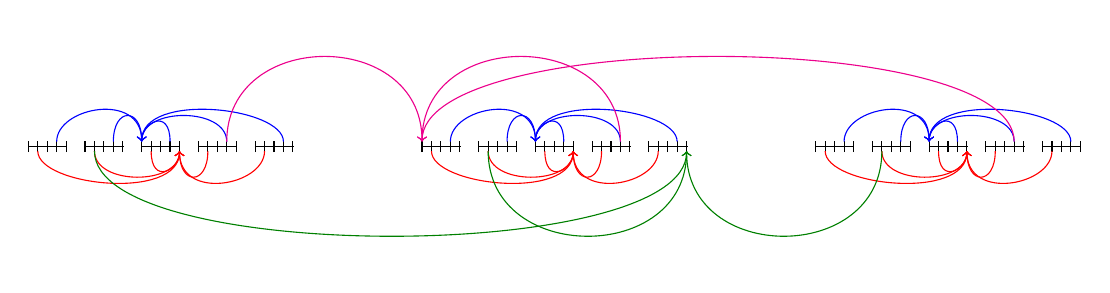
\begin{tikzpicture}
%\def\n{5}\def\np{6} % grid points in nano-patch
\def\n{3}\def\np{4} % grid points in nano-patch
\def\sc{1.2};  % some scaling in horizontal direction
\def\yt{0.06};
% for some things maps index to vertical shift 
\def\y#1{\ifcase#1\or0.7\or0.5\or0.3\or0.5\or0.7\else0\fi}
% maps horizontal nano-patch index to relative horizontal position
%\def\x#1{\ifcase#1\or0\or1\or2\or3\or4\else9\fi}
\def\x#1{\ifcase#1\or0\or0.6\or1.2\or1.8\or2.4\else7\fi}
%
% draw three shifted copies of the micro-patches 
\foreach \s in {0,5,10} {\begin{scope}[shift={(\s,0)}]
%
% draw nano-grid in each nano-patch
\foreach \j in {1,...,5}  {
%	\filldraw[gray!20] (\x\j*\sc,-\yt*\sc) 
%       rectangle (\x\j*\sc+0.\np01*\sc,\yt*\sc);
	\draw[step=0.1*\sc,thin] (\x\j*\sc-0.001*\sc,-\yt*\sc) 
    	grid (\x\j*\sc+0.\np1*\sc,\yt*\sc);
%	\filldraw [red] (\x\j*\sc+\sc*0.1,0) circle (0.5ex); 
%    \draw [red] (\x\j*\sc+\sc*0.\np,0) circle (0.5ex);
%    \node[blue] at (\x\j*\sc,0) {\pgfuseplotmark{triangle}};
%    \node[blue] at (\x\j*\sc+\sc*0.\n,0) {\pgfuseplotmark{triangle*}};
} 
%\pgfsetshortenend{2.0pt}; %because dots are not centred
%about endpoints of lines, but rather end the lines
%
% draw nano-micro coupling interpolation
\foreach \j in {1,...,5} {
    \draw[blue,->] (\x\j*\sc+0.\n*\sc, \yt) 
        .. controls (\x\j*\sc+0.\n*\sc, 0.5) and (\x3*\sc+0.0  *\sc, \y\j)  
        .. (\x3*\sc+0.0  *\sc, \yt);
    \draw[red ,->] (\x\j*\sc+0.1 *\sc,-\yt) 
        .. controls (\x\j*\sc+0.1 *\sc,-0.5) and (\x3*\sc+0.\np*\sc,-\y\j)  
        .. (\x3*\sc+0.\np*\sc,-\yt);
}%end for j
%\pgfsetshortenend{0pt};	
\end{scope} }%end for s shift
%
% draw micro-macro coupling interpolation
\foreach \I in {0,5,10} {
    \draw[green!50!black,->] (\I+\x2*\sc+0.1*\sc,-\yt) 
        .. controls (\I+\x2*\sc+0.1*\sc,-1.5) and (5+\x5*\sc+0.\np*\sc,-1.5)  
        .. (5+\x5*\sc+0.\np*\sc,-\yt);
    \draw[magenta,->] (\I+\x4*\sc+0.\n*\sc,+\yt) 
        .. controls (\I+\x4*\sc+0.\n*\sc,+1.5) and (5+\x1*\sc+0.0*\sc,+1.5)  
        .. (5+\x1*\sc+0.0*\sc,+\yt);
}
\end{tikzpicture}

\paragraph{Heterogeneous diffusion}
For purpose of illustration, say the physical system has an approximately three-periodic nanoscale pattern of diffusivity (between nano-grid points) of the form \(a^*b^*c^*\).
Here the asterisks denote that these diffusivities modulate over the microscale.

Suppose the modulation is such that the diffusivities sampled in the (five) nano-patches within any one micro-patch have the pattern, for example,
\begin{equation*}
abca \quad
a\bar bca \quad
a\bar b\bar ca \quad
ab\bar ca \quad
abca,
\end{equation*}
where \(\bar b\approx b\) and \(\bar c\approx c\).
The period four pattern in the nano-patch system within the micro-patches seems appropriate.

How to couple micro-macro?  That is the question.
It seems to me that we should interpolate from the next-to-edge nanopatches to the opposing edge nanopatches as in the above.
One way might be as drawn above.

But I am have further thoughts: with only five nanopatches, perhaps the period of the microscale heterogeneity should be three nanopatches `wide', not the four that I posited above.  In which case, what?

\end{document}